%Architekturen Echzeit Analyse / Zeitversetzte Analyse
\chapter{Systemarchitekturen}
\label{arch:chapter}
In diesem Kapitel wird folgende Frage beantwortet: \textit{''Wie würde eine Systemarchitektur einer Software aussehen, die die Problemstellung des Auftrags erfüllt?''}.\\

Die Architekturen zeigen verschiedene Lösungsansätze, die mit Hilfe der Analysen im Kapitel \ref{analyse:chapter} entwickelt wurden.\\

Es gibt zwei grundsätzlich verschiedene Lösungsansätze. Hierbei stellt sich die Frage, ob ein sofortiges Eingreifen bei Erkennen einer Malware notwendig ist. Eine Erkennung in Echtzeit bedeutet, dass jedes Netzwerkpaket erst nach einer Überprüfung passieren kann. Bei einer zeitversetzten Erkennung kann es vorkommen, dass ein Paket der Malware aus dem System gelangt, da die Überprüfung erst später erfolgt.


\section{Echtzeit Erkennung}

\begin{figure}[H]
	\centering
	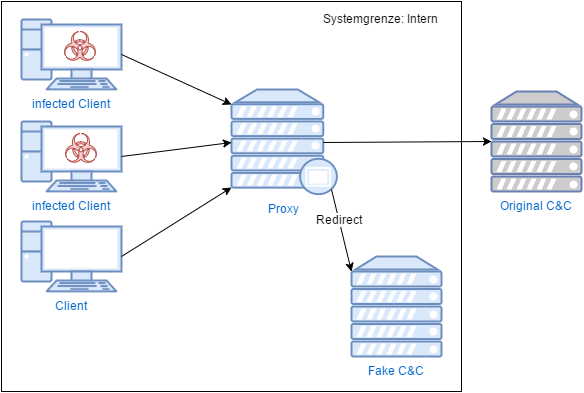
\includegraphics[width=0.85\textwidth]{img/Architektur-EE-A.png}
	\caption{Systemarchitekturen: Echtzeit Erkennung: Systemarchitektur}
	\label{fig:Echtzeit Erkennung: Systemarchitektur}
\end{figure}

Bei der Echtzeit Erkennung befindet sich die gesamte Logik auf dem Proxy. Das Loggen der Pakete fällt weg, weil die Pakete direkt nach Malware Eigenschaften überprüft werden. Falls ein Paket Malware Eigenschaften aufweist, wird es direkt umgeleitet. Diese Methode kann enorme Anforderungen an die Performance stellen, da jedes einzelne Paket überprüft werden muss, bevor es den Proxy passieren darf. Vorteil dieser Architektur ist das sofortige Umleiten, das heisst, dass kein Paket, das Malware Eigenschaften aufweist, jemals den \gls{cc} Server des Angreifers erreichen wird.


\subsection{Malware Detection}
Die Erkennung der Malware Aktivitäten wird durch ein Pattern Matching auf dem Proxy gelöst. Das setzt voraus, dass der Proxy eine Open Source Software ist, oder auf andere Weise das Erweitern ermöglicht.

\subsection{Redirect}
Die Umleitung muss auf Layer 7 geschehen, da die darunter liegenden Layer (z.B. Layer 3) erst beim Versenden durch den Proxy erstellt werden. Eine Umleitung mittels Iptables ist somit nicht möglich. Das erschwert die Implementation dieser Lösung, da diverse Layer 7 Protokolleigenschaften beachtet werden müssen.


\section{Zeitversetzte Erkennung}
Bei der Zeitversetzten Erkennung werden alle Pakete in einer Datenbank gespeichert und dann analysiert, damit man eine Datenbasis zur Analyse besitzt.
Die Kommunikation zwischen Malware und \gls{cc} wird erst bei Erkennen des Patterns umgeleitet.


\subsection{Variante A: Single Proxy}

\begin{figure}[H]
	\centering
	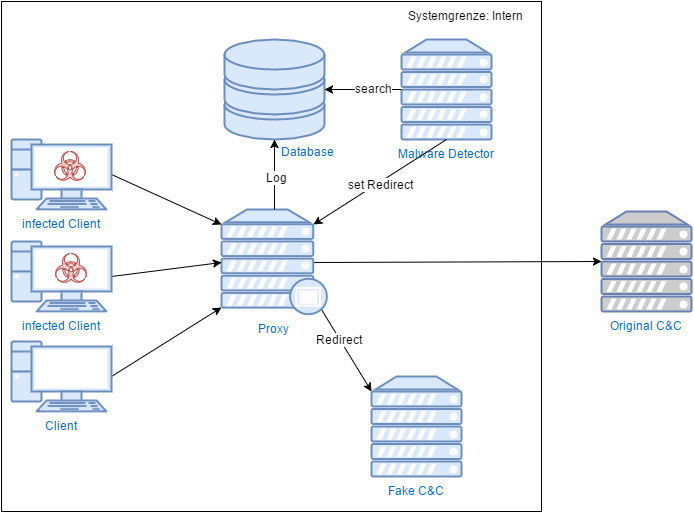
\includegraphics[width=0.85\textwidth]{img/Architektur-ZE-A.png}
	\caption{Systemarchitekturen: Zeitversetzte Erkennung Variante A: Systemarchitektur}
	\label{fig:Zeitversetzte Erkennung Variante A: Systemarchitektur}
\end{figure}

Um die Performance Probleme der Echtzeit Erkennung zu beheben, werden bei der Zeitversetzten Erkennung die Pakete in eine Datenbank geloggt. Das führt dazu, dass die Pakete direkt weitergeleitet werden können. Daraus entsteht jedoch der Nachteil, dass die Pakete einer noch nicht erkannten Malware zum \gls{cc} Server gelangen.

\subsubsection{Logging}
Die geläufigsten Proxies unterstützen \gls{icap}, dass das Loggen des Netzwerkverkehrs auf eine Datenbank ermöglicht. Die Unterstützung von \gls{icap} ist bei dieser Variante eine zwingende Anforderung.

\subsubsection{Malware Detection}
Ein Malware Detector iteriert durch die Datenbank, bei Erkennen einer Malware wird ein Redirect angefordert. Die Suche nach der Malware kann auf diverse Arten gelöst werden. Eine Möglichkeit ist das Loggen auf eine Elasticsearch Datenbank. Mit Hilfe von Full Text Search können dann Pakete mit Malware Eigenschaften gefunden werden.

\subsubsection{Redirect}
Die Umleitung lässt sich hier am besten durch Iptables lösen. Die Iptables können direkt auf dem Host der Proxys definiert werden.

\subsection{Variante B: Proxy Chaining}

\begin{figure}[H]
	\centering
	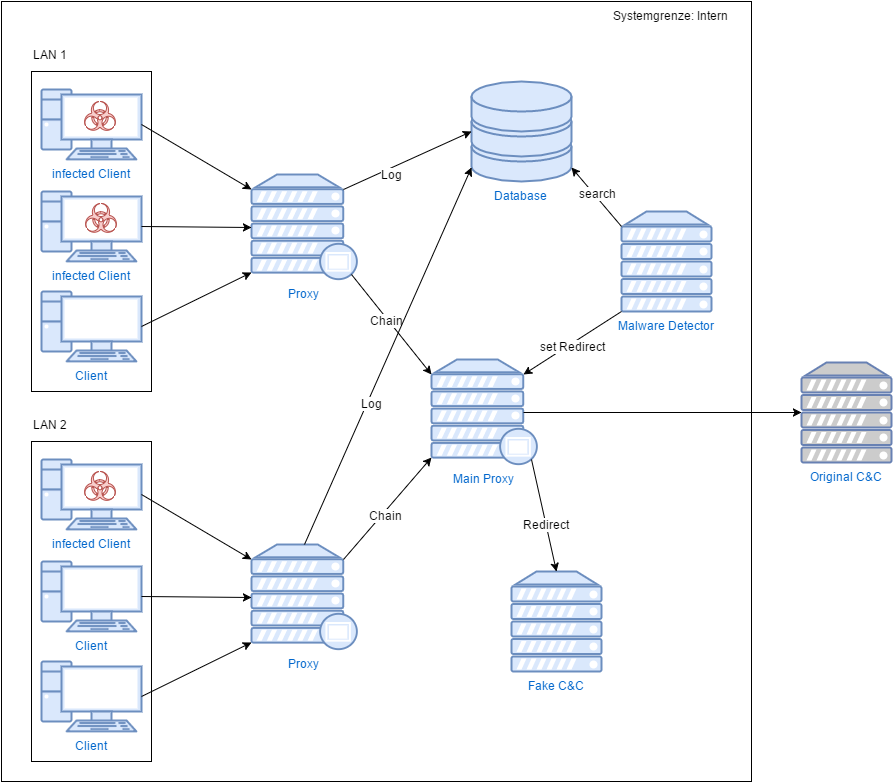
\includegraphics[width=0.85\textwidth]{img/Architektur-ZE-B.png}
	\caption{Systemarchitekturen: Zeitversetzte Erkennung Variante B: Systemarchitektur}
	\label{fig:Zeitversetzte Erkennung Variante B: Systemarchitektur}
\end{figure}

Grössere Firmen besitzen meisstens einen Proxy. Falls der bestehende Proxy keine \gls{icap} Unterstützung aufweist oder ein Logging aus anderen Gründen nicht möglich oder gewünscht ist, bietet diese Architektur eine Lösung. 

\subsubsection{Logging}
Da ein Proxy für das Logging der Pakete benötigt wird, kommt ein Proxy Chaining zum Einsatz. Es können auch mehrere Proxys für verschiedene LANs oder Abteilungen, wie im Diagramm ersichtlich, eingesetzt werden. Diese Proxys loggen die Pakete in eine zentrale Datenbank.

\subsubsection{Malware Detection}
Die Erkennung der Malware ist gleich wie bei Variante A.

\subsubsection{Redirect}
Bei dieser Architektur sind verschiedene Arten des Redirects möglich. Die einfachste Lösung ist eine Iptable hinter oder auf dem letzten Proxy. Im Diagramm wäre das der Main Proxy. Es wäre auch denkbar, den Redirect direkt auf einem der Proxys zu machen, das weist in der Praxis aber Probleme auf.

\subsubsection{\gls{ssl} Bump Problem}
Wenn der Squid Proxy \gls{ssl} Bump aktiviert hat ist dieser nicht fähig nochmals einen CONNECT Request zu einem Upstream Proxy zu machen.
Daher muss der Upstream Proxy bei aktiviertem \gls{ssl} Bump HTTPS unterstützen.

